% Copy to docs/ambiguities/lecture18/main.tex when actual questions arise.
% Replace 18 and the title; add real L18-Qxx entries from the lecture ledger.
% Build from the repository root: make questions LECTURE=18
% Store evidence crops in the new project's images/ folder.
% Questions are for later review. Do not stop transcription or ask live chat
% questions; deliver this PDF with the lecture, keeping unresolved items marked.
\documentclass[a4paper,12pt]{article}
\usepackage[margin=19mm]{geometry}
\usepackage{amsmath,amssymb,graphicx,xcolor}
\usepackage{fontspec}
\usepackage{xepersian}
\settextfont{XB Roya}
\setlatintextfont{Latin Modern Roman}
\definecolor{ink}{HTML}{173D75}
\graphicspath{{images/}}
\setlength{\parindent}{0pt}
\setlength{\parskip}{5pt}
\linespread{1.12}
\newcommand{\qtitle}[2]{{\Large\bfseries\color{ink} پرسش \lr{#1}: #2}\par}
\newcommand{\answer}{\medskip\textbf{پاسخ یا صورت مورد تأیید و تاریخ:}\par\vspace{18mm}\hrule\medskip}
\begin{document}
{\LARGE\bfseries پرسش‌های ابهام جلسهٔ \lr{18}}\par
{\large جزوهٔ جبر پیشرفتهٔ دکتر خسروی}\par
شمارهٔ صفحه‌ها، شمارهٔ یک‌مبنای صفحه در فایل پی‌دی‌اف است، نه شمارهٔ دست‌نویس.
پرسش‌های حل‌نشده هنوز در اسلایدها به‌عنوان متن قطعی پذیرفته نشده‌اند.
\medskip\hrule\medskip

\qtitle{L18-Q01}{حرفِ نام گروه در تعریف بخش‌پذیری}
\textbf{وضعیت:} باز؛ خوانش کاری موقت، بدون پاسخ کاربر. ثبت: ۲۰۲۶/۱۰/۲۵.\par
\textbf{منبع:} نسخهٔ \lr{primary}، صفحهٔ ۱، تعریف بالای صفحه، سطر دوم.
\begin{LTR}\footnotesize\texttt{sources/lectures/18 Injective and Projective Modules 2.pdf}\end{LTR}
\textbf{عبارت منبع:} گروه با حرف $A$ معرفی می‌شود، ولی در شرط، $y\in D$ دیده می‌شود؛ در همان سطر $x\in A$ آمده است.
\begin{center}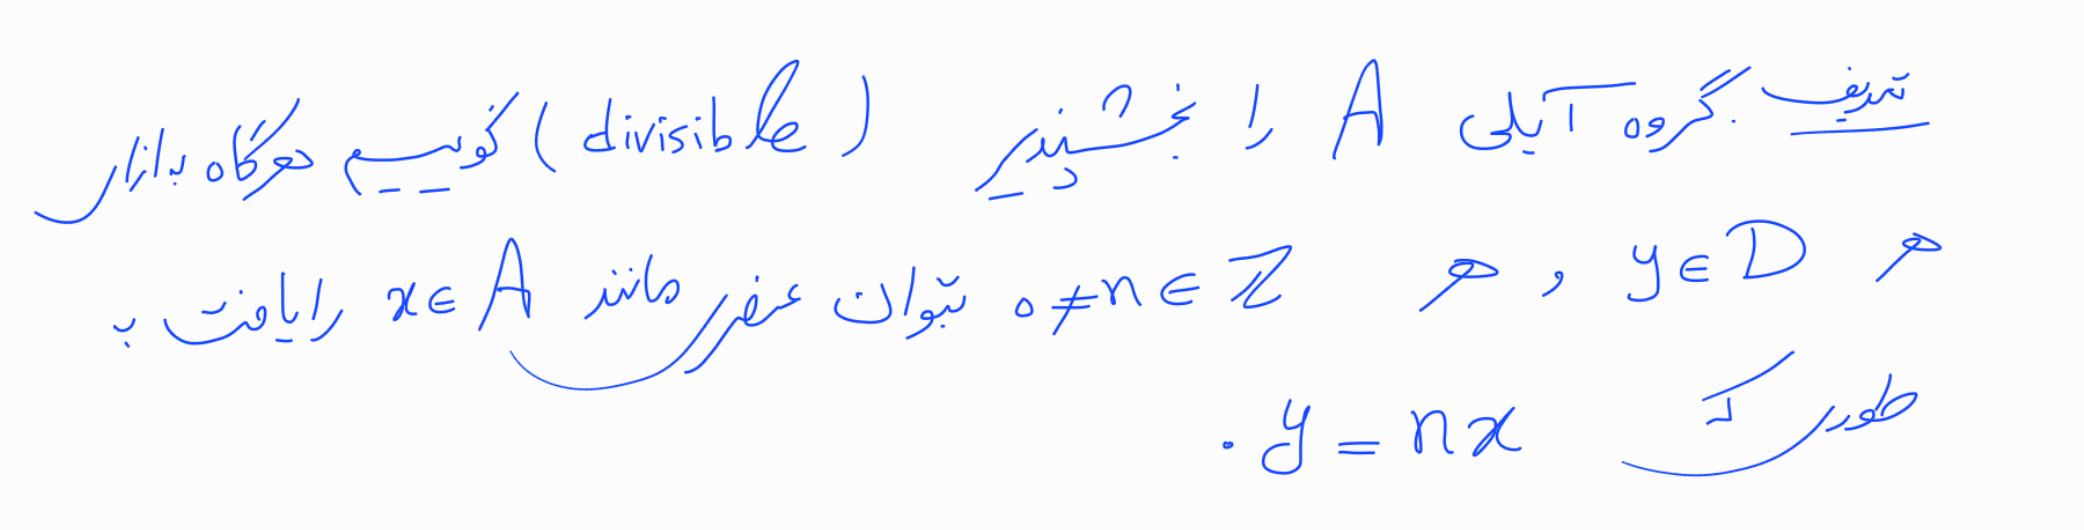
\includegraphics[width=\linewidth]{q01-definition.png}\end{center}
\textbf{خوانش‌های ممکن:} $D$ لغزش قلم به جای $A$ است؛ یا $D$ نام دیگری برای همان گروه است که در این صفحه معرفی نشده؛ یا واقعاً گروهی جداگانه منظور بوده است.
\par
\textbf{شاهد و اثر تفاوت:} در صورت قضیه و هر دو جهت اثبات، فقط $A$ به کار رفته است. اگر $D$ گروهی جدا باشد، جایگاه $y$ و در نتیجه کمیت‌گذارِ تعریف روشن نیست.
\par
\textbf{پرسش برای بازبینی بعدی:} آیا شرط تعریف باید $\forall y\in A$ باشد و حرف $D$ به $A$ تغییر کند؟
\par
\textbf{رفتار در اسلایدها:} در تعریف، $y\in A$ با برچسب «خوانش موقت» آمده است؛ قضیه به همین قرارداد ارجاع می‌دهد. این انتخاب هنوز تأیید کاربر نیست.
\answer

\newpage
\qtitle{L18-Q02}{حالتِ ایده‌آل صفر در اثبات جهت عکس}
\textbf{وضعیت:} باز؛ تکمیلِ حالتِ ایده‌آل صفر موکول به بازبینی است. ثبت: ۲۰۲۶/۱۰/۲۵.\par
\textbf{منبع:} نسخهٔ \lr{primary}، صفحهٔ ۲، از انتخاب $I=(n)$ تا انتخاب $x$ با $f(n)=y=nx$؛ نتیجهٔ انژکتیو بودن در پایین همان برهان.
\begin{LTR}\footnotesize\texttt{sources/lectures/18 Injective and Projective Modules 2.pdf}\end{LTR}
\begin{center}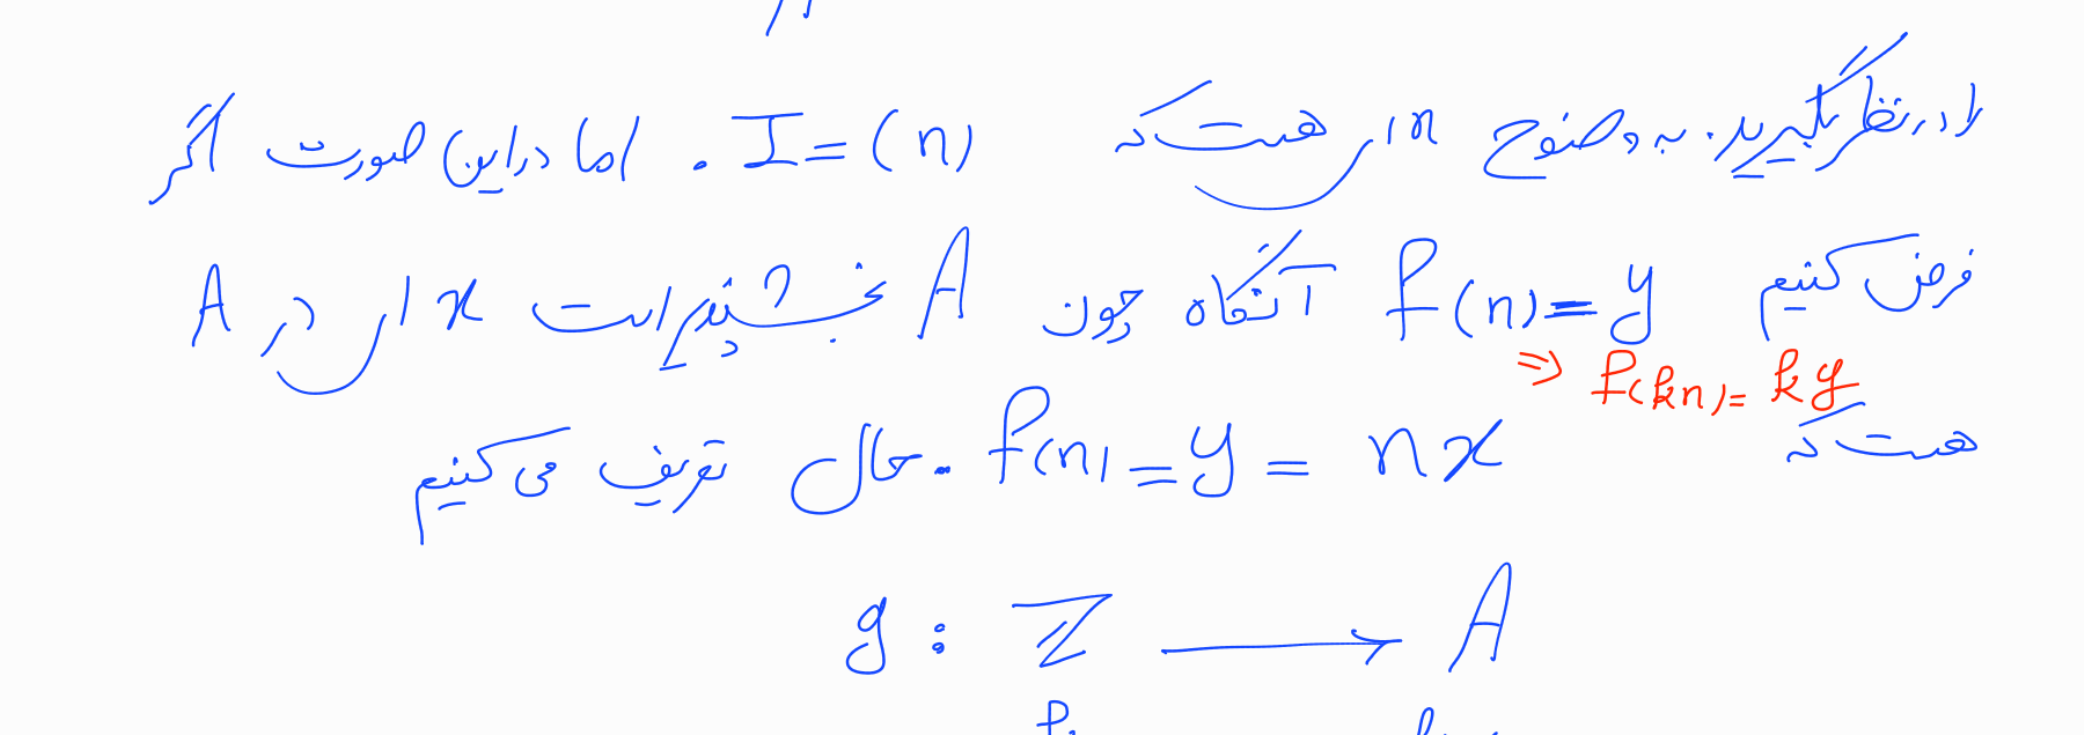
\includegraphics[width=\linewidth]{q02-zero-ideal.png}\end{center}
\textbf{عبارت و شاهد:} $I$ در آغاز ایده‌آلی دلخواه از $\mathbb Z$ است. منبع می‌نویسد $I=(n)$ و سپس از بخش‌پذیری، $f(n)=y=nx$ را به دست می‌آورد؛ اما $n\ne0$ و حالتِ $I=0$ جداگانه ذکر نشده‌اند. تعریفِ بخش‌پذیری در صفحهٔ ۱ فقط برای $n\ne0$ است.
\par
\textbf{خوانش‌های ممکن:} برهان به طور ضمنی فقط ایده‌آل‌های ناصفر را بررسی کرده و حالتِ صفر را بدیهی دانسته است؛ یا فرضِ $n\ne0$ و یک گامِ جدا برای ایده‌آل صفر از یادداشت افتاده است. نمی‌توان کاربرد تعریفِ بخش‌پذیری به $n=0$ را از متن نتیجه گرفت.
\par
\textbf{اثر تفاوت:} معیارِ گسترش از ایده‌آل‌ها، همهٔ ایده‌آل‌ها را شامل می‌شود؛ محاسبهٔ حالت ناصفر به تنهایی تمامِ جهتِ «بخش‌پذیر $\Rightarrow$ انژکتیو» را ثبت نمی‌کند.
\par
\textbf{پرسش برای بازبینی بعدی:} آیا انتخابِ مولد به $n\ne0$ محدود شود و برای $I=0$ گسترشِ صفر به عنوان یک گامِ افزوده و مشخص، جداگانه نوشته شود؟
\par
\textbf{رفتار در اسلایدها:} محاسبهٔ منبع برای $I\ne0$ حفظ شده است. حالتِ صفر و تکمیلِ این جهت از اثبات صریحاً موکول به بازبینی‌اند؛ برهانی از بیرونِ جزوه به عنوان متنِ منبع افزوده نشده است.
\answer

\newpage
\qtitle{L18-Q03}{یکریختیِ خارجی و مکملِ زیرمدولِ مشخص}
\textbf{وضعیت:} باز؛ گام نهاییِ شناساییِ مکمل موکول به بازبینی است. ثبت: ۲۰۲۶/۱۰/۲۵.\par
\textbf{منبع:} نسخهٔ \lr{primary}، صفحهٔ ۷، از انتخاب $\theta:R\to I\oplus R/I$ تا فرمولِ یکی مانده به پایان.
\begin{LTR}\footnotesize\texttt{sources/lectures/18 Injective and Projective Modules 2.pdf}\end{LTR}
\begin{center}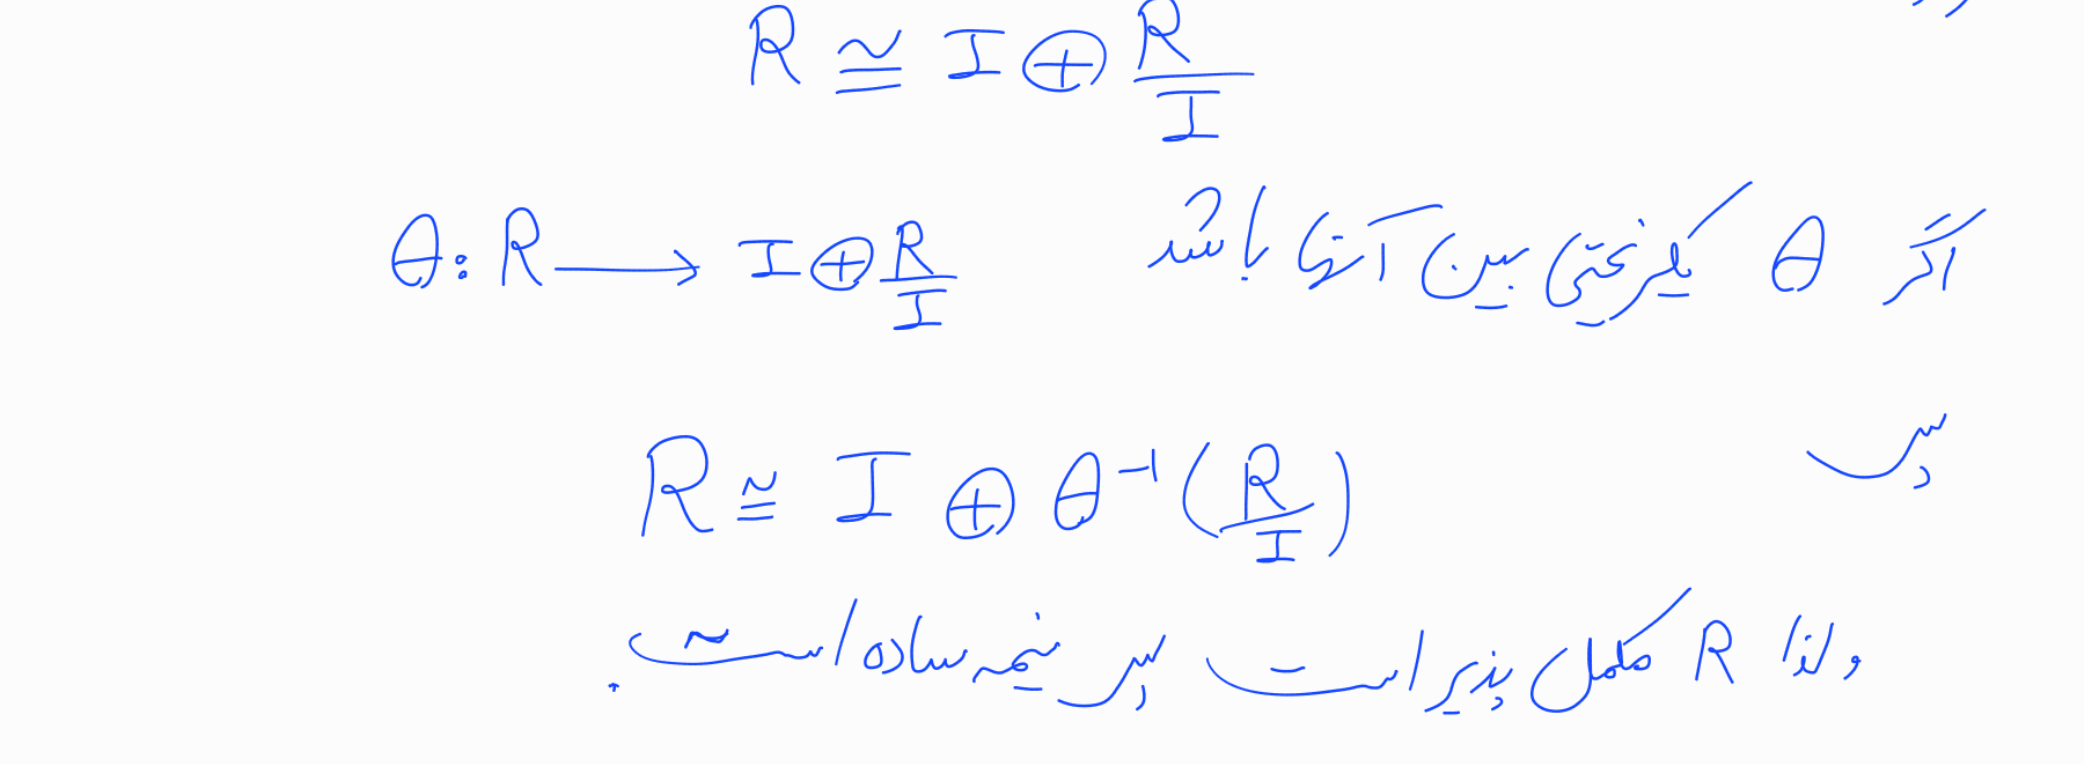
\includegraphics[width=\linewidth]{q03-complement.png}\end{center}
\textbf{عبارت منبع:}
\[
  \theta:R\longrightarrow I\oplus R/I,\qquad
  R\cong I\oplus\theta^{-1}(R/I).
\]
\textbf{خوانش‌های ممکن و شاهد:} رشتهٔ $0\to I\to R\to R/I\to0$ در سطرهای قبل شکافته شده است. ممکن است $\theta$ همان یکریختیِ سازگار با این شکافتن باشد و $R/I$ در فرمول، کوتاه‌شدهٔ $0\oplus R/I$ باشد. اما متن صرفاً یک یکریختی بین دو مدول معرفی می‌کند؛ برای یک یکریختیِ دلخواه، لزوماً $\theta(I)=I\oplus0$ نیست.
\par
\textbf{اثر تفاوت:} برای مکمل‌پذیری، مکملِ همان زیرمدولِ داده‌شدهٔ $I\subseteq R$ لازم است. یک تجزیهٔ خارجی، بدون تعیین سازگاری، این شناسایی را به تنهایی توضیح نمی‌دهد. نمادِ $\cong$ نیز با ادعای جمع مستقیم داخلی یکسان نیست.
\par
\textbf{پرسش برای بازبینی بعدی:} آیا منظور انتخابِ یکریختیِ ناشی از شکافتن با $\theta(I)=I\oplus0$ است و باید نتیجه به صورت
\[
  R=I\oplus\theta^{-1}(0\oplus R/I)
\]
نوشته شود؟ این صورت فعلاً پیشنهادِ توضیح است، نه اصلاحِ تأییدشدهٔ منبع.
\par
\textbf{رفتار در اسلایدها:} فرمولِ لفظیِ منبع و نتیجهٔ ادعاشده حفظ شده‌اند؛ گذار به مکملِ همان $I$ به عنوان گامِ کامل‌شده پذیرفته نشده است.
\answer
\end{document}
